% Created by tikzDevice version 0.12.6 on 2026-10-17 13:58:07
% !TEX encoding = UTF-8 Unicode
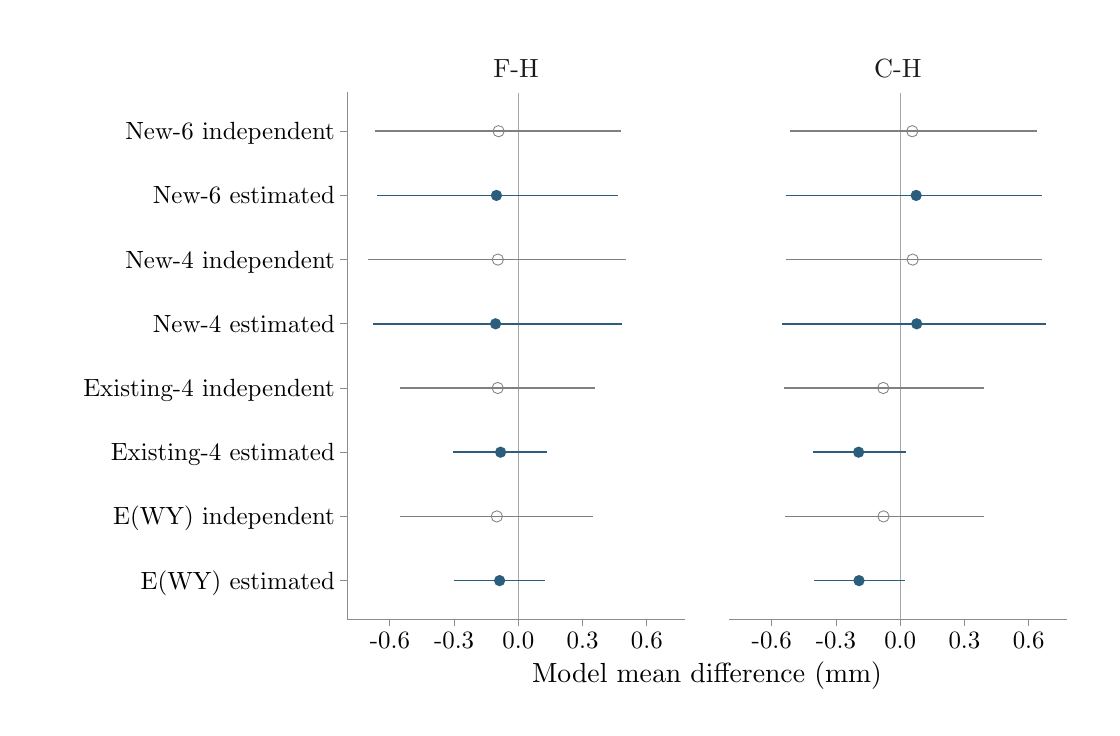
\begin{tikzpicture}[x=1pt,y=1pt]
\definecolor{fillColor}{RGB}{255,255,255}
\path[use as bounding box,fill=fillColor,fill opacity=0.00] (0,0) rectangle (384.48,245.72);
\begin{scope}
\path[clip] (  0.00,  0.00) rectangle (384.48,245.72);
\definecolor{drawColor}{RGB}{255,255,255}
\definecolor{fillColor}{RGB}{255,255,255}

\path[draw=drawColor,line width= 0.5pt,line join=round,line cap=round,fill=fillColor] (  0.00,  0.00) rectangle (384.48,245.72);
\end{scope}
\begin{scope}
\path[clip] (115.51, 31.99) rectangle (237.49,222.22);
\definecolor{fillColor}{RGB}{255,255,255}

\path[fill=fillColor] (115.51, 31.99) rectangle (237.49,222.22);
\definecolor{drawColor}{gray}{0.65}

\path[draw=drawColor,line width= 0.3pt,line join=round] (177.31, 31.99) -- (177.31,222.22);
\definecolor{drawColor}{gray}{0.50}

\path[draw=drawColor,line width= 0.6pt,line join=round] (125.38,208.30) -- (214.57,208.30);

\path[draw=drawColor,line width= 0.6pt,line join=round] (123.00,161.91) -- (216.04,161.91);

\path[draw=drawColor,line width= 0.6pt,line join=round] (134.38,115.51) -- (204.97,115.51);

\path[draw=drawColor,line width= 0.6pt,line join=round] (134.42, 69.11) -- (204.41, 69.11);
\definecolor{drawColor}{RGB}{43,93,125}

\path[draw=drawColor,line width= 0.6pt,line join=round] (126.30,185.10) -- (213.33,185.10);

\path[draw=drawColor,line width= 0.6pt,line join=round] (124.90,138.71) -- (214.70,138.71);

\path[draw=drawColor,line width= 0.6pt,line join=round] (153.85, 92.31) -- (187.75, 92.31);

\path[draw=drawColor,line width= 0.6pt,line join=round] (153.88, 45.91) -- (187.10, 45.91);
\definecolor{drawColor}{gray}{0.50}

\path[draw=drawColor,line width= 0.3pt,line join=round,line cap=round] (170.16,208.30) circle (  2.04);

\path[draw=drawColor,line width= 0.3pt,line join=round,line cap=round] (169.90,161.91) circle (  2.04);

\path[draw=drawColor,line width= 0.3pt,line join=round,line cap=round] (169.85,115.51) circle (  2.04);

\path[draw=drawColor,line width= 0.3pt,line join=round,line cap=round] (169.53, 69.11) circle (  2.04);
\definecolor{fillColor}{RGB}{43,93,125}

\path[fill=fillColor] (169.39,185.10) circle (  2.04);

\path[fill=fillColor] (169.07,138.71) circle (  2.04);

\path[fill=fillColor] (170.89, 92.31) circle (  2.04);

\path[fill=fillColor] (170.53, 45.91) circle (  2.04);
\end{scope}
\begin{scope}
\path[clip] (253.49, 31.99) rectangle (375.48,222.22);
\definecolor{fillColor}{RGB}{255,255,255}

\path[fill=fillColor] (253.49, 31.99) rectangle (375.48,222.22);
\definecolor{drawColor}{gray}{0.65}

\path[draw=drawColor,line width= 0.3pt,line join=round] (315.29, 31.99) -- (315.29,222.22);
\definecolor{drawColor}{gray}{0.50}

\path[draw=drawColor,line width= 0.6pt,line join=round] (275.54,208.30) -- (364.87,208.30);

\path[draw=drawColor,line width= 0.6pt,line join=round] (274.02,161.91) -- (366.37,161.91);

\path[draw=drawColor,line width= 0.6pt,line join=round] (273.16,115.51) -- (345.51,115.51);

\path[draw=drawColor,line width= 0.6pt,line join=round] (273.57, 69.11) -- (345.43, 69.11);
\definecolor{drawColor}{RGB}{43,93,125}

\path[draw=drawColor,line width= 0.6pt,line join=round] (273.92,185.10) -- (366.39,185.10);

\path[draw=drawColor,line width= 0.6pt,line join=round] (272.71,138.71) -- (367.99,138.71);

\path[draw=drawColor,line width= 0.6pt,line join=round] (283.77, 92.31) -- (317.27, 92.31);

\path[draw=drawColor,line width= 0.6pt,line join=round] (284.28, 45.91) -- (317.02, 45.91);
\definecolor{drawColor}{gray}{0.50}

\path[draw=drawColor,line width= 0.3pt,line join=round,line cap=round] (319.65,208.30) circle (  2.04);

\path[draw=drawColor,line width= 0.3pt,line join=round,line cap=round] (319.79,161.91) circle (  2.04);

\path[draw=drawColor,line width= 0.3pt,line join=round,line cap=round] (309.16,115.51) circle (  2.04);

\path[draw=drawColor,line width= 0.3pt,line join=round,line cap=round] (309.25, 69.11) circle (  2.04);
\definecolor{fillColor}{RGB}{43,93,125}

\path[fill=fillColor] (321.06,185.10) circle (  2.04);

\path[fill=fillColor] (321.25,138.71) circle (  2.04);

\path[fill=fillColor] (300.26, 92.31) circle (  2.04);

\path[fill=fillColor] (300.40, 45.91) circle (  2.04);
\end{scope}
\begin{scope}
\path[clip] (115.51,222.22) rectangle (237.49,239.72);
\definecolor{drawColor}{gray}{0.10}

\node[text=drawColor,anchor=base,inner sep=0pt, outer sep=0pt, scale=  0.95] at (176.50,227.71) {F-H};
\end{scope}
\begin{scope}
\path[clip] (253.49,222.22) rectangle (375.48,239.72);
\definecolor{drawColor}{gray}{0.10}

\node[text=drawColor,anchor=base,inner sep=0pt, outer sep=0pt, scale=  0.95] at (314.48,227.71) {C-H};
\end{scope}
\begin{scope}
\path[clip] (  0.00,  0.00) rectangle (384.48,245.72);
\definecolor{drawColor}{gray}{0.55}

\path[draw=drawColor,line width= 0.3pt,line join=round,line cap=rect] (115.51, 31.99) --
	(237.49, 31.99);
\end{scope}
\begin{scope}
\path[clip] (  0.00,  0.00) rectangle (384.48,245.72);
\definecolor{drawColor}{gray}{0.55}

\path[draw=drawColor,line width= 0.3pt,line join=round] (130.89, 29.49) --
	(130.89, 31.99);

\path[draw=drawColor,line width= 0.3pt,line join=round] (154.10, 29.49) --
	(154.10, 31.99);

\path[draw=drawColor,line width= 0.3pt,line join=round] (177.31, 29.49) --
	(177.31, 31.99);

\path[draw=drawColor,line width= 0.3pt,line join=round] (200.52, 29.49) --
	(200.52, 31.99);

\path[draw=drawColor,line width= 0.3pt,line join=round] (223.73, 29.49) --
	(223.73, 31.99);
\end{scope}
\begin{scope}
\path[clip] (  0.00,  0.00) rectangle (384.48,245.72);
\definecolor{drawColor}{RGB}{0,0,0}

\node[text=drawColor,anchor=base,inner sep=0pt, outer sep=0pt, scale=  0.90] at (130.89, 21.31) {-0.6};

\node[text=drawColor,anchor=base,inner sep=0pt, outer sep=0pt, scale=  0.90] at (154.10, 21.31) {-0.3};

\node[text=drawColor,anchor=base,inner sep=0pt, outer sep=0pt, scale=  0.90] at (177.31, 21.31) {0.0};

\node[text=drawColor,anchor=base,inner sep=0pt, outer sep=0pt, scale=  0.90] at (200.52, 21.31) {0.3};

\node[text=drawColor,anchor=base,inner sep=0pt, outer sep=0pt, scale=  0.90] at (223.73, 21.31) {0.6};
\end{scope}
\begin{scope}
\path[clip] (  0.00,  0.00) rectangle (384.48,245.72);
\definecolor{drawColor}{gray}{0.55}

\path[draw=drawColor,line width= 0.3pt,line join=round,line cap=rect] (253.49, 31.99) --
	(375.48, 31.99);
\end{scope}
\begin{scope}
\path[clip] (  0.00,  0.00) rectangle (384.48,245.72);
\definecolor{drawColor}{gray}{0.55}

\path[draw=drawColor,line width= 0.3pt,line join=round] (268.88, 29.49) --
	(268.88, 31.99);

\path[draw=drawColor,line width= 0.3pt,line join=round] (292.08, 29.49) --
	(292.08, 31.99);

\path[draw=drawColor,line width= 0.3pt,line join=round] (315.29, 29.49) --
	(315.29, 31.99);

\path[draw=drawColor,line width= 0.3pt,line join=round] (338.50, 29.49) --
	(338.50, 31.99);

\path[draw=drawColor,line width= 0.3pt,line join=round] (361.71, 29.49) --
	(361.71, 31.99);
\end{scope}
\begin{scope}
\path[clip] (  0.00,  0.00) rectangle (384.48,245.72);
\definecolor{drawColor}{RGB}{0,0,0}

\node[text=drawColor,anchor=base,inner sep=0pt, outer sep=0pt, scale=  0.90] at (268.88, 21.31) {-0.6};

\node[text=drawColor,anchor=base,inner sep=0pt, outer sep=0pt, scale=  0.90] at (292.08, 21.31) {-0.3};

\node[text=drawColor,anchor=base,inner sep=0pt, outer sep=0pt, scale=  0.90] at (315.29, 21.31) {0.0};

\node[text=drawColor,anchor=base,inner sep=0pt, outer sep=0pt, scale=  0.90] at (338.50, 21.31) {0.3};

\node[text=drawColor,anchor=base,inner sep=0pt, outer sep=0pt, scale=  0.90] at (361.71, 21.31) {0.6};
\end{scope}
\begin{scope}
\path[clip] (  0.00,  0.00) rectangle (384.48,245.72);
\definecolor{drawColor}{gray}{0.55}

\path[draw=drawColor,line width= 0.3pt,line join=round,line cap=rect] (115.51, 31.99) --
	(115.51,222.22);
\end{scope}
\begin{scope}
\path[clip] (  0.00,  0.00) rectangle (384.48,245.72);
\definecolor{drawColor}{RGB}{0,0,0}

\node[text=drawColor,anchor=base east,inner sep=0pt, outer sep=0pt, scale=  0.90] at (111.01, 42.82) {E(WY) estimated};

\node[text=drawColor,anchor=base east,inner sep=0pt, outer sep=0pt, scale=  0.90] at (111.01, 66.02) {E(WY) independent};

\node[text=drawColor,anchor=base east,inner sep=0pt, outer sep=0pt, scale=  0.90] at (111.01, 89.22) {Existing-4 estimated};

\node[text=drawColor,anchor=base east,inner sep=0pt, outer sep=0pt, scale=  0.90] at (111.01,112.42) {Existing-4 independent};

\node[text=drawColor,anchor=base east,inner sep=0pt, outer sep=0pt, scale=  0.90] at (111.01,135.61) {New-4 estimated};

\node[text=drawColor,anchor=base east,inner sep=0pt, outer sep=0pt, scale=  0.90] at (111.01,158.81) {New-4 independent};

\node[text=drawColor,anchor=base east,inner sep=0pt, outer sep=0pt, scale=  0.90] at (111.01,182.01) {New-6 estimated};

\node[text=drawColor,anchor=base east,inner sep=0pt, outer sep=0pt, scale=  0.90] at (111.01,205.21) {New-6 independent};
\end{scope}
\begin{scope}
\path[clip] (  0.00,  0.00) rectangle (384.48,245.72);
\definecolor{drawColor}{gray}{0.55}

\path[draw=drawColor,line width= 0.3pt,line join=round] (113.01, 45.91) --
	(115.51, 45.91);

\path[draw=drawColor,line width= 0.3pt,line join=round] (113.01, 69.11) --
	(115.51, 69.11);

\path[draw=drawColor,line width= 0.3pt,line join=round] (113.01, 92.31) --
	(115.51, 92.31);

\path[draw=drawColor,line width= 0.3pt,line join=round] (113.01,115.51) --
	(115.51,115.51);

\path[draw=drawColor,line width= 0.3pt,line join=round] (113.01,138.71) --
	(115.51,138.71);

\path[draw=drawColor,line width= 0.3pt,line join=round] (113.01,161.91) --
	(115.51,161.91);

\path[draw=drawColor,line width= 0.3pt,line join=round] (113.01,185.10) --
	(115.51,185.10);

\path[draw=drawColor,line width= 0.3pt,line join=round] (113.01,208.30) --
	(115.51,208.30);
\end{scope}
\begin{scope}
\path[clip] (  0.00,  0.00) rectangle (384.48,245.72);
\definecolor{drawColor}{RGB}{0,0,0}

\node[text=drawColor,anchor=base,inner sep=0pt, outer sep=0pt, scale=  1.00] at (245.49,  9.13) {Model mean difference (mm)};
\end{scope}
\end{tikzpicture}
